\documentclass{article}
\usepackage{afterpage}
\usepackage{float}
\usepackage{longtable}
\usepackage{graphicx}
\usepackage{pdflscape}
\usepackage[numbers,sort&compress]{natbib}
\usepackage{psfrag}

\usepackage{amsmath}
\usepackage{amsfonts}
\usepackage{graphicx}
\usepackage{nicefrac}
\usepackage{graphicx}
\usepackage{caption}
% \usepackage{subcaption}
\usepackage{subfigure}
% \usepackage{algorithm}
% \usepackage{paralist}
% % \usepackage[geometry]{ifsym}
\usepackage{rotating}
%
\newcommand{\nedelec}{N\'{e}d\'{e}lec }

\newcommand{\uu}[1]{\boldsymbol #1}
\usepackage{listings}
\usepackage{xcolor}
\lstset{language=C++,
                keywordstyle=\color{blue},
                stringstyle=\color{red},
                commentstyle=\color{green},
                morecomment=[l][\color{magenta}]{\#}
}
\begin{document}

\section*{MHD - Neumann bilinear form}

The variational for the MHD model with inhomogeneous Neumann conditions is
\begin{equation}
\label{eq:VariationForm}
\begin{split}
A(\uu{u}_h,\uu{v}) + O(\uu{u}_h;\uu{u}_h,\uu{v}) +C(\uu{b}_h;\uu{v},\uu{b}_h) +B(\uu{v}, p_h) & =  (\uu{f},\uu{v})_\Omega - (\uu{p_N},v)_{\Omega_N}\\
B(\uu{u}_h,q)&= 0, \\
M(\uu{b}_h,\uu{c})-C(\uu{b}_h;\uu{u}_h,\uu{c})+ D(\uu{c},r_h)&= (\uu{g},\uu{c})_\Omega,\\
D(\uu{b}_h,s)&=0,
\end{split}
\end{equation}
where $\uu{p_N}$ is the Neumann condition. Then the Picard iteration is given by:
\begin{equation}
\label{eq:picard}
\begin{split}
A(\delta\uu{u}_h, \uu{v}) +O({\uu{u}_h};\delta\uu{u}_h,\uu{v})+ C(\uu{b}_h;\uu{v},\delta \uu{u}_h) + B(\uu{v}, \delta p_h) & = R_u(\uu{u}_h,\uu{b}_h,p_h;\uu{v}),\\
B(\delta\uu{u}_h,q)&= R_p(\uu{u}_h;q),\\
M(\delta \uu{b}_h,\uu{c})+
D(\uu{c},\delta r_h)-C(\uu{b}_h;\delta \uu{u}_h,\uu{v})&= R_b(\uu{u}_h,\uu{b}_h,r_h;\uu{c}),\\
D(\delta \uu{b}_h,s)&= R_r(\uu{b}_h;s),
\end{split}
\end{equation}
where
\begin{equation}
\label{eq:RHSpicard}
\begin{split}
 R_u(\uu{u}_h,\uu{b}_h,p_h;\uu{v})=&(\uu{f}, \uu{v})_\Omega- (\uu{p_N},v)_{\Omega_N}-A(\uu{u}_h,\uu{v})
-  O(\uu{u}_h;\uu{u}_h,\uu{v})\\
& - C(\uu{b}_h;\uu{v},\uu{b}_h)-B(\uu{v},p_h),\\
R_p(\uu{u}_h;q)=&-B(\uu{u}_h,q),\\
 R_b(\uu{u}_h,\uu{b}_h,r_h;\uu{c})=&(\uu{g,c})_\Omega -M(\uu{b}_h,\uu{c})
+ C(\uu{b}_h;\uu{u}_h,\uu{c})-D(\uu{c},r_h),\\
R_r(\uu{b}_h;s)=&-D(\uu{b}_h,s),
\end{split}
\end{equation}
Therefore you need to enforce the inhomogeneous Neumann conditions at each non-linear iteration???? Also, if you enforce homogeneous boundary conditions within the non-linear iteration doesn't this stop model from capturing the pressure driven flow?

A final thought, the expression for $\uu{p_N}$ is linear and hence would arise in its original form throughout the non-linear iterations.

\section*{MHD - smooth Neumann conditions}

Consider the exact solution:
\begin{figure}[h!]
    \centering
    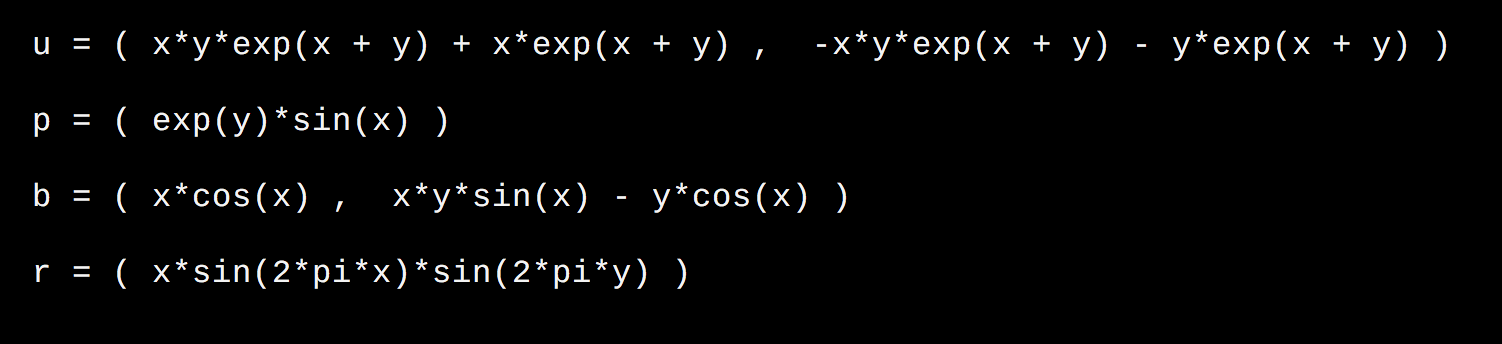
\includegraphics[width=\textwidth]{Solution}
\end{figure}


The error tables are given below. Here I used a unit square domain with Neumann conditions on the left and right boundaries and Dirichlet on the top and bottom ones.
\begin{table}[h!]
\begin{center}
\begin{tabular}{cccccccc}
\hline \hline

$\ell$ &    Dofs $\uu{u}_h/p_h$ & $\|\uu{e}_u\|_{L^2(\Omega)}$ & $r$ & $\|\uu{e}_u\|_{H^1(\Omega)}$ & $r$ &$\|e_p\|_{L^2(\Omega)}$ & $r$  \\
\hline
\hline
1 &      50/9 &  9.0942e-02 &     - &  1.2457e+00 &     - &  5.6315e-01 &      - \\
2 &     162/25 &  1.1441e-02 &     3.53 &  3.2338e-01 &     2.29 &  7.8755e-02 &      3.85 \\
3 &     578/81 &  1.3656e-03 &     3.34 &  8.1946e-02 &     2.16 &  9.2087e-03 &      3.65 \\
4 &    2,178/289 &  1.6719e-04 &     3.17 &  2.0637e-02 &     2.08 &  1.0929e-03 &      3.35 \\
5 &    8,450/1,089 &  2.0858e-05 &     3.07 &  5.1826e-03 &     2.04 &  1.6142e-04 &      2.88 \\
6 &   33,282/4,225 &  2.6265e-06 &     3.02 &  1.2990e-03 &     2.02 &  3.1921e-05 &      2.39 \\
7 &  132,098/16,641 &  2.7450e-07 &     3.28 &  3.2522e-04 &     2.01 &  7.4632e-06 &      2.12 \\
\hline\hline
\end{tabular}

\caption{Convergence for 2D MHD - fluid variables}
\label{tab:MHD_2D_smooth_fluids_velocity}
\end{center}
\end{table}


\begin{table}[h!]
\begin{center}
\begin{tabular}{cccccccccc}
\hline
\hline
$\ell$ &    Dofs $\uu{b}_h/r_h$ & $\|\uu{e}_b\|_{L^2(\Omega)}$ & $l$ & $\|\uu{e}_b\|_{H({\rm curl},\Omega)}$ & $l$ \\
\hline\hline
 1 &     16/9 &  1.8060e-01 &     - &  2.6788e-01 &        - \\
 2 &     56/25 &  9.1265e-02 &     1.09 &  1.3398e-01 &        1.11 \\
 3 &    208/81 &  4.5753e-02 &     1.05 &  6.7003e-02 &        1.06 \\
 4 &    800/289 &  2.2892e-02 &     1.03 &  3.3503e-02 &        1.03 \\
 5 &   3,136/1,089 &  1.1448e-02 &     1.01 &  1.6752e-02 &        1.01 \\
 6 &  12,416/4,225 &  5.7241e-03 &     1.01 &  8.3759e-03 &        1.01 \\
 7 &  49,408/16,641 &  2.8621e-03 &     1.00 &  4.1879e-03 &        1.00 \\
\hline\hline

\end{tabular}
\caption{Convergence for 2D MHD  - magnetic variable}
\label{tab:MHD_2D_smooth_magnetic}
\end{center}
\end{table}



\begin{table}[h!]
\begin{center}
\begin{tabular}{cccccccccc}
\hline
\hline
$\ell$ &    Dofs $\uu{b}_h/r_h$ & $\|\uu{e}_r\|_{L^2(\Omega)}$ & $l$ & $\|\uu{e}_r\|_{H^1(\Omega)}$ & $l$ \\
\hline\hline
  1 &     16/9 &  2.7524e-01 &     - &  2.4780e+00 &     - \\
  2 &     56/25 &  1.4850e-01 &     1.21 &  1.7787e+00 &     0.65 \\
  3 &    208/81 &  4.8879e-02 &     1.89 &  1.0042e+00 &     0.97 \\
  4 &    800/289 &  1.3198e-02 &     2.06 &  5.1942e-01 &     1.04 \\
  5 &   3,136/1,089 &  3.3659e-03 &     2.06 &  2.6198e-01 &     1.03 \\
  6 &  12,416/4,225 &  8.4572e-04 &     2.04 &  1.3128e-01 &     1.02 \\
  7 &  49,408/16,641 &  2.1170e-04 &     2.02 &  6.5676e-02 &     1.01 \\
\hline\hline

\end{tabular}
\caption{Convergence for 2D MHD  - multiplier variable}
\label{tab:MHD_2D_smooth_multiplier}
\end{center}
\end{table}


\newpage

\section*{MHD - Hartmann Neumann conditions}


Consider the exact solution:
\begin{figure}[h!]
    \centering
    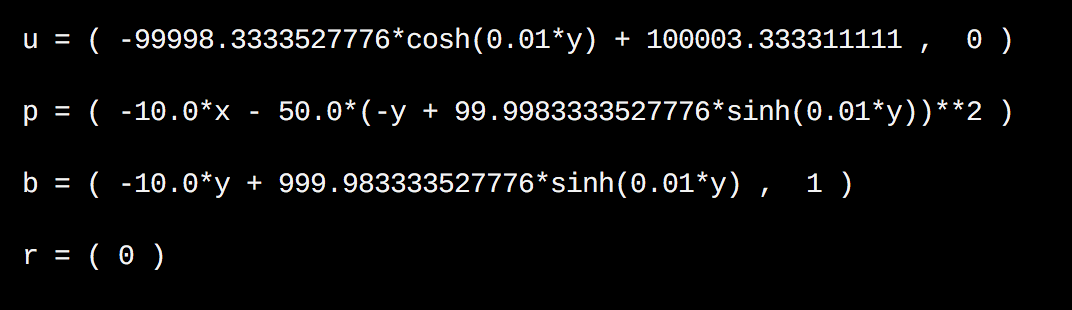
\includegraphics[width=\textwidth]{HartmannSol}
\end{figure}
I have considered exactly the same parameter setup as in your CNAME paper.


\subsection*{Small domain - $(0,1)\times(0,1)$}
\begin{table}[h!]
\begin{center}
\begin{tabular}{cccccccc}
\hline \hline

$\ell$ &    Dofs $\uu{u}_h/p_h$ & $\|\uu{e}_u\|_{L^2(\Omega)}$ & $r$ & $\|\uu{e}_u\|_{H^1(\Omega)}$ & $r$ &$\|e_p\|_{L^2(\Omega)}$ & $r$  \\
\hline
\hline
1 &      50/9 &  1.0907e-06 &     - &  5.9809e-06 &     - &  6.8112e-07 &      - \\
2 &     162/25 &  2.4709e-07 &     2.53 &  1.5978e-06 &     2.25 &  1.1813e-07 &      3.43 \\
3 &     578/81 &  1.2943e-07 &     1.02 &  4.0806e-07 &     2.15 &  9.4741e-08 &      0.38 \\
4 &    2,178/289 &  1.6700e-07 &     0.38 &  1.0278e-07 &     2.08 &  1.0221e-07 &      0.12 \\
5 &    8,450/1,089 &  1.5944e-07 &     0.07 &  2.5669e-08 &     2.05 &  1.0260e-07 &      0.01 \\
6 &   33,282/4,225 &  1.6102e-07 &     0.01 &  7.1451e-09 &     1.87 &  1.0227e-07 &      0.00 \\
7 &  132,098/16,641 &  1.6184e-07 &     0.01 &  5.4389e-09 &     0.40 &  1.0223e-07 &      0.00 \\
\hline\hline
\end{tabular}

\caption{Convergence for 2D MHD - fluid variables - small domain}
\label{tab:MHD_2D_smooth_fluids_velocity}
\end{center}
\end{table}



\begin{table}[h!]
\begin{center}
\begin{tabular}{cccccccccc}
\hline
\hline
$\ell$ &    Dofs $\uu{b}_h/r_h$ & $\|\uu{e}_b\|_{L^2(\Omega)}$ & $l$ & $\|\uu{e}_b\|_{H({\rm curl},\Omega)}$ & $l$ &$\|\uu{e}_r\|_{L^2(\Omega)}$ \\
\hline\hline

 1 &     16/9 &  2.0609e-05 &     - &  6.6536e-05 &        - & 7.9542e-18 \\
 2 &     56/25 &  1.0642e-05 &     1.06 &  3.3834e-05 &        1.08 & 1.0057e-11 \\
 3 &    208/81 &  5.3645e-06 &     1.04 &  1.6987e-05 &        1.05 & 7.6667e-11 \\
 4 &    800/289 &  2.6877e-06 &     1.03 &  8.5022e-06 &        1.03 & 4.6064e-10 \\
 5 &   3,136/1,089 &  1.3445e-06 &     1.01 &  4.2522e-06 &        1.01 & 5.5048e-09 \\
 6 &  12,416/4,225 &  6.7236e-07 &     1.01 &  2.1262e-06 &        1.01 & 6.7659e-08 \\
 7 &  49,408/16,641 &  3.3619e-07 &     1.00 &  1.0631e-06 &        1.00 & 4.2016e-07 \\
\hline\hline

\end{tabular}
\caption{Convergence for 2D MHD  - magnetic variable - small domain}
\label{tab:MHD_2D_smooth_magnetic}
\end{center}
\end{table}


\newpage

\subsection*{Original domain - $(0,10)\times(1,1)$}


\begin{table}[h!]
\begin{center}
\begin{tabular}{cccccccc}
\hline \hline

$\ell$ &    Dofs $\uu{u}_h/p_h$ & $\|\uu{e}_u\|_{L^2(\Omega)}$ & $r$ & $\|\uu{e}_u\|_{H^1(\Omega)}$ & $r$ &$\|e_p\|_{L^2(\Omega)}$ & $r$  \\
\hline
\hline
1 &     210/33 &  8.4039e-05 &     - &  1.5327e-04 &     - &  1.2410e-05 &      - \\
2 &     738/105 &  2.2328e-05 &     2.11 &  4.2124e-05 &     2.06 &  3.1605e-06 &      2.36 \\
3 &    2,754/369 &  5.6093e-06 &     2.10 &  1.0752e-05 &     2.07 &  4.5085e-06 &      0.57 \\
4 &   10,626/1,377 &  1.2471e-06 &     2.23 &  2.7021e-06 &     2.05 &  4.5568e-06 &      0.02 \\
5 &   41,730/5,313 &  6.6421e-07 &     0.92 &  6.7647e-07 &     2.02 &  4.5738e-06 &      0.01 \\
6 &  165,378/20,865 &  7.1821e-07 &     0.11 &  1.6886e-07 &     2.02 &  4.5791e-06 &      0.00 \\

\hline\hline
\end{tabular}

\caption{Convergence for 2D MHD - fluid variables - original domain}
\label{tab:MHD_2D_smooth_fluids_velocity}
\end{center}
\end{table}



\begin{table}[h!]
\begin{center}
\begin{tabular}{cccccccccc}
\hline
\hline
$\ell$ &    Dofs $\uu{b}_h/r_h$ & $\|\uu{e}_b\|_{L^2(\Omega)}$ & $l$ & $\|\uu{e}_b\|_{H({\rm curl},\Omega)}$ & $l$ &$\|\uu{e}_r\|_{L^2(\Omega)}$ \\
\hline\hline

1 &     72/33 &  1.5144e-04 &     - &  5.5277e-04 &        - &   8.9585e-16\\
2 &    264/105 &  9.0833e-05 &     0.79 &  2.9756e-04 &        0.95 &   2.0906e-15\\
3 &   1,008/369 &  4.7431e-05 &     0.97 &  1.5131e-04 &        1.01 &   2.3104e-15\\
4 &   3,936/1,377 &  2.3971e-05 &     1.00 &  7.5968e-05 &        1.01 &   3.1749e-15\\
5 &  15,552/5,313 &  1.2017e-05 &     1.01 &  3.8023e-05 &        1.01 &   4.8842e-15\\
6 &  61,824/20,865 &  6.0127e-06 &     1.00 &  1.9016e-05 &        1.00 &   5.7900e-15\\
\hline\hline

\end{tabular}
\caption{Convergence for 2D MHD  - magnetic variable - original domain}
\label{tab:MHD_2D_smooth_magnetic}
\end{center}
\end{table}

\newpage

\subsection*{Large domain - $(0,80)\times(1,1)$}


\begin{table}[h!]
\begin{center}
\begin{tabular}{cccccccc}
\hline \hline

$\ell$ &    Dofs $\uu{u}_h/p_h$ & $\|\uu{e}_u\|_{L^2(\Omega)}$ & $r$ & $\|\uu{e}_u\|_{H^1(\Omega)}$ & $r$ &$\|e_p\|_{L^2(\Omega)}$ & $r$  \\
\hline
\hline
 1 &    490/75 &  4.2854e-03 &     - &  3.9356e-03 &     - &  3.3003e-04 &      - \\
 2 &   1746/245 &  1.1348e-03 &     2.09 &  1.0919e-03 &     2.02 &  9.2882e-05 &      2.14 \\
 3 &   6,562/873 &  2.8863e-04 &     2.07 &  2.7938e-04 &     2.06 &  6.7975e-05 &      0.49 \\
 4 &  25,410/3,281 &  7.1669e-05 &     2.06 &  6.8712e-05 &     2.07 &  7.2061e-05 &      0.09 \\
 5 &  99,970/12,705 &  1.7437e-05 &     2.06 &  1.7137e-05 &     2.03 &  7.2392e-05 &      0.01 \\

\hline\hline
\end{tabular}

\caption{Convergence for 2D MHD - fluid variables - large domain}
\label{tab:MHD_2D_smooth_fluids_velocity}
\end{center}
\end{table}



\begin{table}[h!]
\begin{center}
\begin{tabular}{cccccccccc}
\hline
\hline
$\ell$ &    Dofs $\uu{b}_h/r_h$ & $\|\uu{e}_b\|_{L^2(\Omega)}$ & $l$ & $\|\uu{e}_b\|_{H({\rm curl},\Omega)}$ & $l$ &$\|\uu{e}_r\|_{L^2(\Omega)}$ \\
\hline\hline

 1 &    170/75 &  5.6497e-03 &     - &  6.9921e-03 &        - & 3.0388e-14\\
 2 &    628/245 &  3.1297e-03 &     0.90 &  3.7639e-03 &        0.95 & 3.5901e-14\\
 3 &   2,408/873 &  1.6074e-03 &     0.99 &  1.9140e-03 &        1.01 & 5.2011e-14\\
 4 &   9,424/3,281 &  8.0912e-04 &     1.01 &  9.6096e-04 &        1.01 & 6.6039e-14\\
 5 &  37,280/12,705 &  4.0524e-04 &     1.01 &  4.8097e-04 &        1.01 & 1.0988e-13\\

\hline\hline


\end{tabular}
\caption{Convergence for 2D MHD  - magnetic variable - large domain}
\label{tab:MHD_2D_smooth_magnetic}
\end{center}
\end{table}


\subsection*{Discussion}

\begin{itemize}
  \item I have a working smooth solution model with Neumann boundary conditions - see "MHD - smooth Neumann conditions" section. The convergence rates are what we would expect for a smooth solution here.
  \item For the Hartmann flow example if have produced tables for three separate domains (small, original and large). In each case, the errors are small for the first mesh level, $\ell$.
  \item I have decreased the Picard tolerance to 1e-10 but I still get the same error convergence results.
  \item For the original and large meshes it is possible to see that the fluid variables start to exhibit the correct convergence results. However, $\|\uu{e}_u\|_{L^2(\Omega)}$ appears to be an order less than we would expect.
  \item Recall that we are using TH P2/P1 for the fluid variables and N1/P1 mixed \nedelec approximation for the magnetic variables. Could the loss in order in $\|\uu{e}_u\|_{L^2(\Omega)}$ be a result of the miss match in the orders of the velocity and magnetic fields??

\end{itemize}

\end{document}

